%%%%%%%%%%%%%%%%%%%%%%%%%%%%%%%%%%%%%%%%%%%%%%%%%%%%%%%%%%%%%%%%%%%%%%%%%%%%%%%%%%%%%%%%%%%%%%%%%%%%%%%%%%%%%%%%%%%%%%%%%%%%%%%%%%%%%%%%%
\section{Path selection}\label{sec:esnr_pathsel}
While today's access point and wireless distribution system (WDS) infrastructure networks use tree-structured topologies and have only a single path between any two nodes, a future device-to-device wireless network such as Wi-Fi Direct may offer many paths along which packets can be routed. Choosing which path in a multi-hop wireless network will provide the best throughput is the \define{path selection} problem, and it can be thought of as a generalization of the access point selection problem I described in \secref{sec:esnr_apsel}. Indeed, a client implicitly makes a routing decision when joining a WDS network---which access point it chooses can make a large difference in its connection quality to the root access point that serves Internet access. Research in multi-hop routing for wireless mesh networks~\cite{Bahl_repeater,Rodrig_thesis} has shown that the choice of path can effect a large difference in connection quality.

The practical state of the art in this area is the recent work by Bahl et al.~\cite{Bahl_repeater} on an opportunistic repeater scheme for 802.11a. In this design, when a client with a strong link detects rate anomaly~\cite{Heusse_RateAnomaly}---that is, that its throughput is hurt by a client with a weak link monopolizing airtime---the strong client evaluates whether relaying that client's packets would improve throughout for both. In certain scenarios, they showed that this could improve aggregate performance of the network by 50\%--200\%.

While this solution is practical and works well, the use of new techniques in 802.11n significantly complicates the picture. First, the scheme of Bahl et al.\ uses a link's RSSI (as a measure of Packet SNR) to select between the 8 available 802.11a rates. In contrast, as I have shown in \chapref{chap:delivery}, Packet SNR does not accurately predict the rate for 802.11n links, nor does it enable devices to choose between different MIMO modes. Second, Bahl et al.\ used a homogenous network of single-antenna 802.11a chipsets; but the set of devices in 802.11n networks will be heterogeneous and support differing numbers of antennas and asymmetric transmit/receive capabilities. While it is not clear how to handle these challenges via the Packet SNR, the Effective SNR offers the ability to overcome them. In this section, I evaluate the ability of Effective SNR to deliver the benefits of opportunistic repeaters in 802.11n networks.

Note that the problem of path selection does not differ significantly from that of AP selection, except that when choosing between repeaters (or a direct link) the entire path must be considered rather than merely the last hop. For simplicity, I assume that the network diameter is small such that pipelining~\cite{Rodrig_thesis} is of limited benefit, and do not consider schemes that forward along multiple unreliable paths such as ExOR~\cite{Biswas_ExOR}. I next describe the basic path selection algorithm I evaluate and characterize the multi-hop paths in my testbed.

%Instead, in this section I focus on how 802.11n and heterogeneous devices change the opportunities available from relaying, and whether Effective SNR delivers these improvements.

\subsection{Path selection algorithm}
%%%%%%%%%%%%%%%%%%%%%%%%%%%%%%%%%%%%%%%%%%%%%%%%
\begin{algorithm}[tp]
\caption{\label{alg:relay_sel_basic}\fcall{RelaySelection(Relay Set $R$, Source $s$, Destination $d$)}}
\begin{algorithmic}[1]
\STATE $t_\text{direct} \gets 1/\fcall{PredictBitrate}(s,d)$ \COMMENT{time to send a bit directly from $s$ to $d$, or $\infty$}
\FORALL {$r \in R$}
\STATE \emph{// time to hop through $r$ is the sum of the times of the two hops}
\STATE $t_{\text{relay},r} \gets 1/\fcall{PredictBitrate}(s,r) + 1/\fcall{PredictBitrate}(r,d)$
\ENDFOR
\STATE $r_\text{opt} \gets \argmin_{r\in R} t_{\text{relay},r}$ \COMMENT{find the optimal relay $r_\text{opt}$ with the shortest path}
\IF {$t_{\text{relay},r_\text{opt}} < t_\text{direct}$}
\RETURN $r_\text{opt}$ \COMMENT{if optimal relay offers a shorter path}
\ELSE
\RETURN $\emptyset$ \COMMENT{if the direct link is best}
\ENDIF
\end{algorithmic}
\end{algorithm}
%%%%%%%%%%%%%%%%%%%%%%%%%%%%%%%%%%%%%%%%%%%%%%%%

I describe a simplified path selection algorithm in \algref{alg:relay_sel_basic}. This \define{relay selection} algorithm only considers paths with a single intermediate node (called a \define{relay}). In step 4, this algorithm computes the \define{expected transmission time (ETT)}~\cite{Draves_ETT} of the multi-hop path as the sum of the time to transfer the packet along each hop. This metric makes the optimistic assumption that there is no protocol overhead, and hence provides an overestimate of actual performance, but lets us compare the ability of Packet SNR and Effective SNR algorithms to inform these choices. To balance this optimism, I only consider paths that provide at least 20\% throughput improvement over a direct link.

Relay selection is only a subset of the full path selection problem, but it is simple and recoups much of the potential gain. I considered all $24*23*11=6072$ source-destination-channel tuples in the UW testbed, where I consider each 5\GHz channel as a different instantiation of the network. Of these 6072 node pairs, 2037 (34\%) have a direct link. Adding in optimal one-hop relays enables a further 2317 (38\%) of node pairs to connect, for a total of 4354 (72\%) connected links. The remaining 1713 (28\%) of node pairs require two relays to connect, and would probably be best helped by switching to the 2.4\GHz band in order to obtain higher SNR and longer links.

How much can relaying help in this testbed? To evaluate this, I calculated the bitrate of the optimal one-hop relay choice. I also computed the bitrate of the optimal path using a modification of \algref{alg:relay_sel_basic} to handle multiple hops. (Note that, because it ignores overheads that increase roughly linear in the number of hops, the path bitrate is even more optimistic than the relay bitrate.)

\begin{figure}[t]
\begin{minipage}{0.48\textwidth}
	\centering
	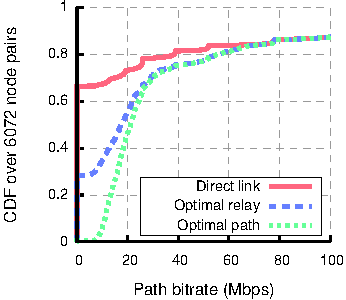
\includegraphics[width=\textwidth]{figures/applications/relay_gains.pdf}
	\caption{\label{fig:relay_sel_gains}Performance of the direct link and the optimal relay or multi-hop path.}
\end{minipage}
\hfill
\begin{minipage}{0.48\textwidth}
	\centering
	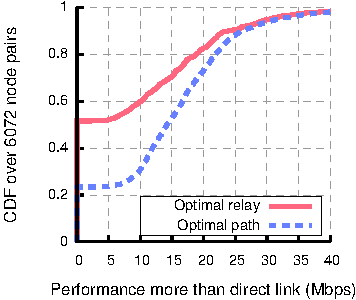
\includegraphics[width=\textwidth]{figures/applications/relay_gains_mbps.pdf}
	\caption{\label{fig:relay_sel_gains_mbps}Performance gain from relay or multi-hop path.}
\end{minipage}
\end{figure}

\figref{fig:relay_sel_gains} shows the net bitrate of the direct link, optimal relay, or best multi-hop path between the 6072 node pairs. This figure demonstrates that the use of a single relay captures most of the improvement for node pairs that can communicate faster than 20\Mbps. Though the relay strategy leaves a quarter of the node pairs disconnected, the optimal multi-hop paths only enable those nodes to communicate at an optimistic estimate of 10--20\Mbps over 3 or more hops. In practice, the benefits to these node pairs would likely be small.

\figref{fig:relay_sel_gains_mbps} shows the achievable improvement in bitrate between the node pairs. Only 25\% (1621/6072) of node pairs gain 20\Mbps or more using these strategies, and 60\% (964) of these also gain 20\Mbps using a single relay.

As these results show that relay selection recoups most of the gains of full path selection in this testbed, I restrict the path selection problem to selecting a good relay for the rest of this section. To complete the description of the algorithms, I now explain how to choose relays using Effective SNR and Packet SNR. To complete \algref{alg:relay_sel_basic}, we need only define the function \fcall{PredictBitrate}, which we use to predict the bitrate of the link studied.

\subsubsection{Relay selection with Effective SNR}
To define the function \fcall{PredictBitrate} for Effective SNR, we can simply use \fcall{GetMetric-EffectiveSNR} (\algref{alg:eff_snr_link_metric})---because the link metric of interest for Effective SNR is indeed simply the predicted bitrate of the link.

\subsubsection{Relay selection with Packet SNR}
Unfortunately, defining a \fcall{PredictBitrate-EffectiveSNR} function for Packet SNR is trickier. We have already seen in \chapref{chap:delivery} that Packet SNR is not a good indicator of packet delivery for a specific MCS, so we can't use the approach we used for Effective SNR in \algref{alg:eff_snr_link_metric}. But there should still be a positively correlated relationship between Packet SNR and expected bitrate, which I use instead to predict the bitrate. (Note that this will not tell \emph{which} specific modulation and coding schemes to use, only what the expected bitrate will be among the many choices.)

\begin{figure}[t]
	\centering
	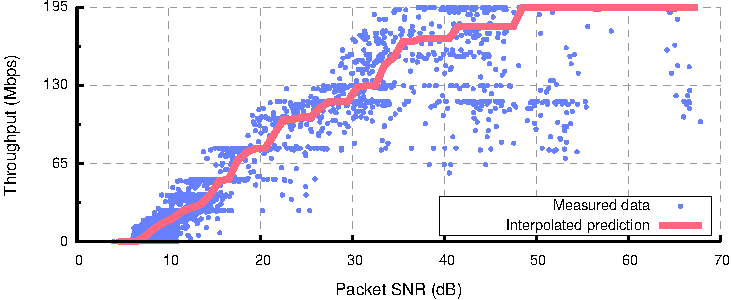
\includegraphics[width=\textwidth]{figures/applications/snr_vs_mbps.pdf}
	\caption{\label{fig:snr_vs_mbps}Deriving a prediction for throughput as a function of Packet SNR.}
\end{figure}

To generate this function, measured the optimal throughput and Packet SNR for all the links in my testbed. I then divided this data into 1\dB-wide SNR bins, and took the median throughput of each bin as the throughput prediction for that Packet SNR value. By connecting these medians (and dropping some sparse bins with so that the line monotonically increases), I derived a monotonic function that uses the Packet SNR measurement to predict the throughput of a link. I plot the original data as a scatterplot in \figref{fig:snr_vs_mbps}, with the interpolated throughput prediction also shown as a solid line. To define \fcall{PredictBitrate-PacketSNR} in order to define a Packet SNR-based relay selection algorithm, I simply look up the Packet SNR of the link and return the throughput predicted by this line.

Having defined both algorithms for relay selection, I next evaluate their performance.

\begin{figure}[t]
	\centering
	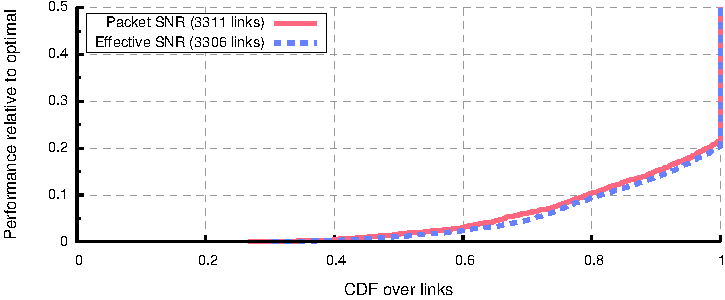
\includegraphics[width=\textwidth]{figures/applications/relay_ratio_opt.pdf}
	\caption{\label{fig:relay_ratio_opt}Relay selection algorithm performance relative to an optimal algorithm.}
\end{figure}
\begin{figure}[t]
	\centering
	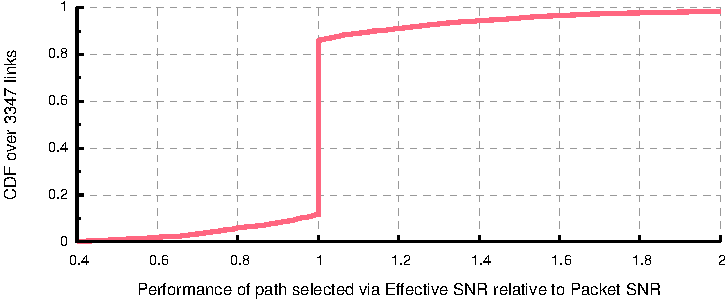
\includegraphics[width=\textwidth]{figures/applications/relay_ratio.pdf}
	\caption{\label{fig:relay_ratio}The relative throughput selecting relays by Packet SNR or by Effective SNR}
\end{figure}

\subsection{Relay selection performance}
I evaluated the performance of \algref{alg:relay_sel_basic} using Packet SNR or Effective SNR to predict performance on the same dataset.

\figref{fig:relay_ratio_opt} plots the relative performance of each algorithm to the optimal relay algorithm, and has a truncated $y$-axis. Note that the algorithms, which choose to use a relay or not based on predictions of performance, do not choose to use a relay for the same number or set of links. Taking the union of the links for which either algorithm chooses a relay, \figref{fig:relay_ratio} shows the ratio of the path chosen using Effective SNR to the path chosen with Packet SNR. Both algorithms perform very well, choosing an optimal relay in 80\% of cases.

The head-to-head comparison shows a potentially surprising result: the Packet SNR and Effective SNR-based algorithms have nearly indistinguishable performance. Effective SNR chooses a better path for 473/3347 (14\%) of links and a worse path for 393 (12\%), but this is a tiny (2.4\%) difference overall. The Effective SNR and Packet SNR lines in \figref{fig:relay_ratio_opt} are nearly indistinguishable. Unlike for access point or channel selection, the ability of Effective SNR to account for subchannel effects does not improve performance over simply using Packet SNR for relay selection.

To explain this phenomenon, recall from \figref{fig:relay_sel_gains} that the links for which performance improves using a relay are those links with low speeds (somewhat less than 100\Mbps). This is because the best possible relay path---a path with two maximum-rate hops (195\Mbps)---would have an idealized rate of 97.5\Mbps. Consequently, direct links that are faster will not benefit from a one-hop relay. Then, these results indicate that the interpolated throughput values in \figref{fig:snr_vs_mbps} are fairly accurate for slower links.

Why would Packet SNR accurately predict the expected performance for slower links? I offer two explanations. First, note that the throughput prediction task that I use to select paths is easier than the packet delivery (\chapref{chap:delivery}) or rate selection problems (\chapref{chap:rate}). Rather than knowing which rate particular configuration points work to provide the best performance, the algorithm need simply predict the expected performance value. This statistical property is easier to get right, and need not be exact in order to find a good path: a slight over- or under-estimate of one or both hops might not change the final path selection. For example, if a hop delivers about 78\Mbps, it does not matter whether this is achieved as \mcs{12} (two streams at 39\Mbps each) or \mcs{19} (three streams at 25\Mbps each). Similarly, for a path using two 78\Mbps hops (total idealized throughput 39\Mbps), an erroneous prediction of 65\Mbps for one hop results in an estimate of 35.5\Mbps which is close to the truth and might still lead to a correct relay selection.

Secondly, slower links are likely to be using single-stream SIMO or dual-stream MIMO2 configurations rather than the three streams used to achieve the absolute fastest rates. The packet delivery results in \chapref{chap:delivery}, particularly as demonstrated by \figref{fig:snr_rate_step_1x3} and \figref{fig:snr_rate_step_2x3}, showed that Packet SNR can be fairly accurate for these configurations, which exploit spatial diversity using the excess receive antennas.

These two factors combined explain why Packet SNR performs well for relay selection in my testbed. This property should generalize, as relaying is generally most useful for slow links. Effective SNR simply offers little gain in this application. Still, Effective SNR performs as well as Packet SNR (if not slightly better) and given its other benefits is a natural fit for this application. %It will also be important in heterogeneous networks where not all relays support the same number of antennas.

%\subsection{Measurements on 802.11a vs 802.11n}
%Denote node in center of testbed as AP, and pick a channel. Consider nodes in decreasing order of RSS: have them associate to the network, then turn into repeaters from which the next node can choose. Assume optimal decisions are made at each step. Compare 1x1, 1x3, and 3x3 versions of this scenario.
%\begin{itemize}
%\item What is the distribution of distance (\#hops) from each node to AP? [How often is repeating used, and at what scale?]
%\item What is the distribution of end-to-end tpt? Of the fraction of max (i.e., 65\Mbps or 195\Mbps)? Of the improvement? [This gets at whether the gains get larger or smaller with various device changes.]
%\end{itemize}
%Same scenario with randomly assigned 3x3, 2x3, and 1x3 devices. How does heterogeneity affect these results?
%
%\subsection{Measurements of Effective SNR}
%Perform the same experiments as described above, this time predicting rate by RSSI and then by Effective SNR\@. (Use this only for topology choice, but assume rate selection finds the correct rate.)